\chapter{Verification and testing}
\label{cha:testing}

	\section{Functional requirements verification}
A key aspect of the DRI service is to meet its requirements within Cloud
Platform, which were listed in section \ref{requirements}. In the prototype
phase, we are focusing mostly on data validation. As project continues, data
replication mechanisms will be developed within DRI service. As previous
chapters shown, we designed and implemented a service which enables periodic
and on-request data validation and notifies about any integrity or availability
errors. It can be used according to the REST interface described in chapter
\ref{cha:architecture}.\\

In future Cloud Platform releases Notification Service depicted in figure
\ref{fig:dri-architecture} will provide notification functionalities for the
platform. In our prototype, we developed simple mock for this important
component in the form of a webpage. Its sample view during normal operation is
presented in figure \ref{fig:notification-service}.

\begin{figure}[h!]
	\centering
	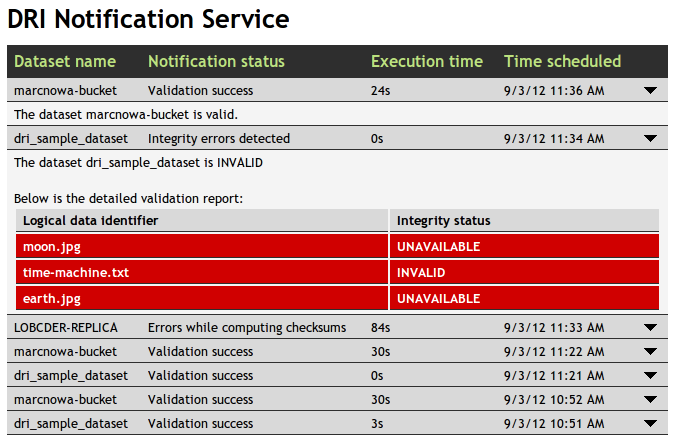
\includegraphics[width=0.8\textwidth]{images/notification-service.png}
	\caption{Notification service mock -- sample view}
	\label{fig:notification-service}
\end{figure}

Here we can see a tabular view of the notifications. Each notification
initially is presented as one row. Each row shows basic information: dataset
which
 
	\section{Efficiency metrics}
		\subsection{Network bandwidth}
		\subsection{Error detection rate}
		\subsection{Scalability}
	\section{Efficiency tests}
		\subsection{Environment description}
		\subsection{Experiments}
		\subsection{Results}
	\section{Other nonfunctional requirements verification}
	\section{Conclusions and results}
